\chapter{Secure Information Flow Analysis of Python Programs}
There have been many studies on information flow control and all of them share some basic properties like information flow should be from less secure entity to more secure entity. Denning's book \cite{denning} has a chapter on information flow control, this chapter describes lattice model for information flow \cite{lattice}, this makes it easy to track information flow in a program using transitivity property. Analysis has been done on basic operations which involve information flow like assignment operation (explicit flow) based on data flow, conditional operations like if else, while etc. (implicit flows) based on control flow, information flow through covert channel based on traps and exception in programs. Here are some basic rules given in \cite{denning}, (arrow $\rightarrow$ denotes information flow).  
\begin{itemize}
	\item x = y : y $\rightarrow$ x
	\item if e then x = y : e $\rightarrow$ x
	\item while w {if e then{ x = y} w =false } : w $\oplus$ e $\rightarrow$ x
	\item infinite loop: while w {}; x = y :- w $\rightarrow$ x etc.   
\end{itemize}
Chen et al. \cite{hybrid}(published in 2014) presented work on python byte-code and claimed that there was no work related to python at that time. They implemented information flow checker for python byte-code using static and dynamic analysis but their main focus is on information flow policies related to objects. Kumar et al. \cite{rwfm} introduce a new model to work with subjects and my work will be focused on this. Conti et al. \cite{taint} provide library support in python for information flow analysis in explicit flows only.
Data Security can be achieved using information flow policies. Execution of any action
like copying of file, read operation on file or memory, write operation on file or memory, execution of statement etc may cause flow of information. Usually, information revealed that was
unknown before execution of statement termed as information flow otherwise if it was known already then there will be no information flow. This thesis focuses on information flow between
variables used in a python program irrespective of the amount of information flowing. There are two kinds of information flow among variables:\\
\begin{enumerate}
	\item{\textbf{Explicit Information Flow}}\\
	\begin{lstlisting}[language=Python, caption=Python example]
	x = y
	x = math.log(y)\end{lstlisting}
	these assignment operations are example of explicit flow because information related to variable y is flowing into x using data dependency in both cases.
	\item{\textbf{Implicit Information Flow}}\\
	\begin{lstlisting}[language=Python, caption=Python example]
	if y == 1:
	x = 1
	\end{lstlisting}
	\pagebreak
	\begin{lstlisting}[language=Python, caption=Python example, label=lst:whilecode]
	while y < z:
	x = 1
	y += 1\end{lstlisting}
	in these examples value of x after execution of statements depends on the control path
	taken by the program, variable y and z used in choosing between two control path in while
	program, this involvement of y and z in making decision reduce the uncertainty of variables
	y and z. Whether y < z or y > z can be observed with help of final value of x after execution of given code in listing \ref{lst:whilecode} . So there is indirect implicit flow from y to x in the first example and implicit flow from y
	and z to x in the second example\cite{denning}.\\~\\
	\begin{lstlisting}[language=Python, caption=Python example, label=lst:infwhile]
	x = 0
	while y == 1:
	pass
	x = 1\end{lstlisting}
	Here assignment operation on x in Listing \ref{lst:infwhile} is outside of while body but still information flowing from y to x because execution of x = 1 statement depends on termination of while loop, so you can know value of y by checking the value of x after execution of program, for example if value of x is 1 and program terminated then y must be other than 1, if while loop goes in infinite loop then y must be 1.
	
	The first chapter describes python program certification with the help of Denning's Lattice Model. The lowest security class in this lattice assumed is Low everyone can read information from this class, the highest class in the lattice is High, 
	information from all security classes can flow into it but no information can flow from this class to others.
	For Example certification of python code in Listing \ref{lst:lattice} needs to follow Denning's lattice and constraints written in figure \ref{fig:lattice}, security class of variable var is denoted by \dud{var}.  
	\begin{lstlisting}[language=Python,caption={Python example}, label={lst:lattice}]
	x = 0
	z = 1
	y = 0
	if x :
	while z :
	y = 1\end{lstlisting}
	\begin{figure*}[h]
		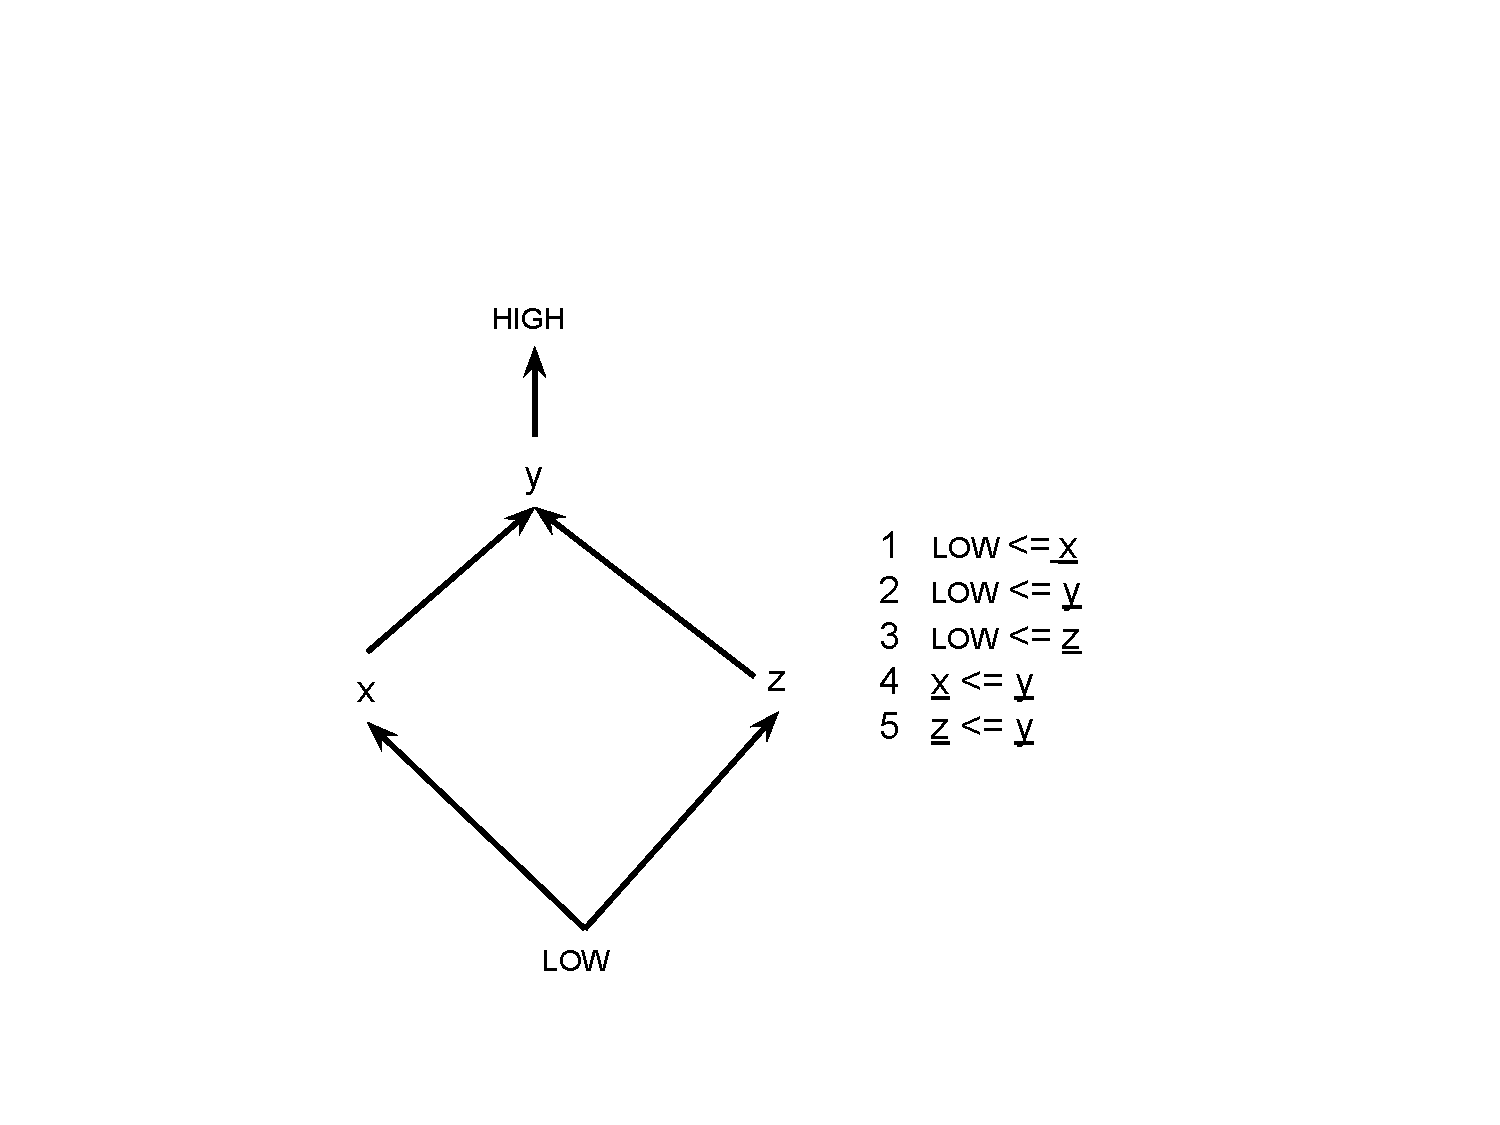
\includegraphics[width=0.6\textwidth]{lattice}
		\centering
		\caption{Lattice of Listing \ref{lst:lattice}}
		\label{fig:lattice}
	\end{figure*}
	Chapter \ref{ch:caseStudy} describes information flow by nonterminating while loop and how to certify program in such situation.
	Chapter \ref{ch:caseStudy} describes how information flows among thread in the multi-threaded program using semaphore.
	Chapter \ref{ch:constgen} presents a new approach to certifying a program using more sophisticated labels (RWFM label)
	and it also considers subjects for certification of the program.	
\end{enumerate}     

